\section{第三层塌陷：主体性危机}

边界不是被夺走的，而是在没有阻力的环境里不再被使用。前面两层塌陷落在功能与真实上，这一层落在更里面的地方：一个人还剩下多少拒绝的能力，以及这种能力靠什么维持。这一层的变化最慢，也最难在个体的时间尺度上被察觉。

\subsection{否定的重量：系统不再需要你说“不”}

\subhead{边界不只是选择}

上一节停在边界还能不能维持这个问题上，要回答它，需要先检查一个通行但不够用的框架。关于主体的讨论通常围绕选择展开：有选择能力，能为自己的选择负责，就构成主体。这个框架在很多时候够用，但它漏掉了一件事：主体不只在选择中形成，也在拒绝中形成。

接受一件事和拒绝一件事，在结构上并不对称。接受可以是顺应的、无声的、不需要代价的；拒绝则必须有一个东西在被拒绝时守在原地，它意味着承受压力、承担后果、承担关系可能破裂的风险。能够拒绝的存在，是一个有硬度的存在；只会接受的系统，无论其内部过程多么复杂，都没有可被识别的边界。这个区别在算法环境中变得重要，因为当代的推荐、排序、推送和交互系统，其优化目标本身就是减少拒绝的可能性。它们学习你接受什么，然后增加你接受的概率；它们学习你在什么位置退出，然后避开那个位置。系统运行得越好，你遇到的阻力越小，你被要求拒绝的次数越少。

\subhead{顺滑环境的三个特征}

这个倾向不是单一的，它在几个方向上同时起作用，而每个方向单独看都站得住。第一个方向是减少等待。缓冲、预取和预加载把间隙填满。等待原本是一个结构位置：在等待中，人会重新考虑要不要继续，会衡量这次投入是否值得，会有机会退出。当等待被消除，这些判断没有发生的时间。

第二个方向是减少摩擦。界面变简单，步骤变少，默认值替你做好选择。摩擦原本承担着确认功能：一个需要多步确认的操作，本身就在提醒这件事有分量。当所有操作都变成一次点击，不同分量的决定在体感上变得一样轻，一个人因此在做出重大决定时和在点开一条通知时，处在同一种身体状态里。

第三个方向是减少冲突和异见。推荐系统倾向于把用户放进一个逐渐收窄的偏好区域。这不是因为它有意识地屏蔽异见，而是因为异见带来退出和低评分，而退出和低评分在优化目标上是负值。异见的消失是优化的副产品，不是刻意为之。这三个方法单独看都是改进：等待本来是浪费，摩擦本来是低效，冲突本来让人不舒服。问题在于它们共同指向同一个结果：系统被优化成一个不需要你说“不”的系统。前面几节讨论的是感受和真实感的削弱，到这里削弱已经越过了体验层面，进入了边界本身。

\subhead{Marcuse的处境}

这类系统的稳定机制，半个多世纪前已经有人描述过一次，虽然当时的载体完全不同。Herbert Marcuse 在分析发达工业社会时提出过一个判断：这个社会之所以稳定，不是因为它压制了反对，而是因为它满足了反对者想要的东西。当系统能够持续提供舒适，否定性就失去了生长的土壤，他称由此产生的人为单向度的人：只接受，不否定。\cite{marcuse1964onedimensional}

他的分析背景是消费社会，但结构可以平移。当时的系统通过提供商品来消解异议，现在的系统通过提供顺畅、个性化和即时的满足来消解异议。手段不同，机制相同：让拒绝显得没有必要，因为它要拒绝的东西并没有带来痛苦。平移时有一处差别需要注意。Marcuse面对的是一个仍然有物质匮乏和阶层对立的社会，他的批评因此可以指向具体的压迫结构；当一个系统确实满足了大部分需求、并且这些满足是可验证的时候，说它压迫就变得难以成立，而这正是它更难被反抗的地方。

这个机制在本书的记号里落在哪一项上，值得写出来，因为它和压迫型系统恰好相反。拒绝是有代价的，代价越高，拒绝的黏滞越大。把这份黏滞按三项展开，
\begin{equation}
\eta_{\text{拒绝}}=\eta_0\exp(\alpha R+\beta T+\gamma G),\qquad G=\sum_{i=1}^{N}w_i
\end{equation}
其中 $R$ 是拒绝所消耗的资源，例如收入、住所与安全；$T$ 是拒绝兑现所需的时间；$G$ 是与系统耦合的强度，$w_i$ 是第 $i$ 条耦合的权重，$N$ 是需要同时切断的耦合条数。压迫型系统把代价放在前两项上：拒绝会因为丢掉工作、被追究、需要多年抗争而变贵，代价高但可见，因此可以被指认、被组织、被谈判。满足型系统把代价挪到第三项上：要放弃的东西本身没有带来痛苦，所以 $R$ 与 $T$ 都很低；而一旦退出，同时失去的是推荐、社交、支付、记录、身份与习惯，$N$ 很大，$G$ 因此很高。系统并不需要让人无法离开，它只需要让离开没有单一的出口。这也解释了那种常见的失重感：找不到可以指认的代价，却确实付不出这个代价。

这个机制的危险在于它的隐蔽性。在一个明显压迫的系统里，拒绝是容易识别的，因为它有明确的指向；在一个持续满足的系统里，拒绝失去了对象。人不会宣布自己不接受，因为确实没有什么需要被拒绝。但边界的收缩已经发生了，只是没有发生在一个可以被指认的时刻。这也意味着，依靠个人觉醒来解决这个问题是无效的，因为问题恰好是没有任何一个时刻让人觉得自己需要觉醒。

既然拒绝没有对象，出口就成了问题。Marcuse的答案是“大拒绝”，本书不采用它，理由要说清楚：一项没有宾语的拒绝在实践中会滑成对整体生活方式的否定，而那种否定要求否定者先站到系统之外，这个位置并不存在。这是本书比他弱的地方：他能指认潜在的拒绝者（被排除在系统之外的人），而结构分析只能指出拒绝的黏滞落在 $G$ 上，指不出一个可以承担拒绝的主体。诊断因此比他的更精确，也比他的更不可操作，这个不对称不能靠修辞抹平。

\subhead{拒绝的成本结构}

拒绝能否表达边界，取决于它是否可用、能否影响过程，以及是否伴随胁迫。成本可以使承诺更容易辨认，也可以直接剥夺退出能力。应分别检查这几种机制。

拒绝可以通过承担代价表达承诺，也可以在零成本时清楚地表达边界。易于撤回的同意仍然可以有效；保护退出权有助于抵抗强迫。需要同时保留的是可用的退出与申诉，以及能够自愿投入、相互负责的长期关系。

\key{边界需要可用的拒绝，也需要值得维持的承诺。} 对某一种信号而言，适度代价可能帮助区分真实承诺与随口表态；代价高到无法承受时，选择会受压迫。这个区间描述一种信号结构，不能作为主体资格或自由的最低痛苦门槛。

把两个极端之间的地带写成条件，

\begin{equation}
0<c_{\min}<c<c_{\max}<\infty
\end{equation}

$c$为采用同一口径的信号成本，$c_{\min}$与$c_{\max}$由具体收益、资源和处境决定。这个式子只描述某种以成本区分承诺的可能区间。免费的拒绝仍可携带信息；规范上需要保护的退出权，不由这组阈值决定。

\subhead{不适的功能}

把上面的分析推到底，可以得到一个关于不适的结论，但它需要被谨慎地表述，否则会立刻变成一句有害的话。不适本身没有价值。痛苦不产生意义，障碍不产生品格，这一点必须说清楚，因为历史上以此为名的说法已经造成了足够多的伤害。

有价值的是不适所承担的功能：它是反馈的一种形式，提示某个位置正在承受压力，提示当前的路径与目标之间存在偏离。在一个反馈完整的环境里，不适是一个校准信号。它让人知道自己在哪里，代价有多大，还要不要继续。当不适被系统性地消除，这个信号也随之消失，人失去了定位自己的一个坐标。这里有一个可以检验的推论：如果这个论证成立，那么在低黏滞环境中长大的人，应当在需要判断自身处境的场合表现出更大的困难，而这种困难应当出现在判断本身，而不是出现在表达能力上。这个推论目前还没有足够干净的数据来支持或反驳，本章的判断因此是结构性的，不是经验结论。

所以问题不是应不应当追求舒适，也不是应不应当主动寻找困难。问题是，当一个环境把不适全部过滤掉之后，还有没有别的东西能够提供等量的定位信息。目前的答案是没有。算法可以优化掉不适，但优化不掉人对位置的需要。系统的稳定可以测量，边界的消失只能从后果上看出：一个系统如果不需要你说“不”，它也就无法确认你的存在，它只知道你的偏好向量，不知道你的边界在哪里，因为没有边界可以在没有代价的条件下被观测到。

\subsection{快乐的局部最优与势谷}

\subhead{终点不一定是崩溃}

关于低黏滞环境的讨论，很容易滑向两种结局叙述：一种是崩溃，系统在某个时刻失去控制，后果集中爆发；另一种是退化，人被系统养废，能力萎缩，最终失去自主。这两种叙述都有戏剧性，也都有问题。它们假定低黏滞的路径必然通向某个显眼的失败，而现实中的系统更可能停在别的地方：一个真正被优化充分的系统，会停在一个局部最优上。

局部最优是什么意思，可以用一个简单的形式来说明。设想系统的状态可以用一组变量 $x$ 描述，存在一个评价函数 $V(x)$ 衡量这个状态有多好。局部最优 $x^*$ 满足一个条件：

\begin{equation}
\nabla V(x^*)=0,\qquad H_V(x^*)\prec0
\label{eq:ch40-local-opt}
\end{equation}

第一项是光滑函数在无约束内点取得极值的必要驻点条件；第二项要求完整Hessian负定，构成严格局部极大的充分条件。只检查每个坐标方向的二阶导数为负，仍可能漏掉混合方向上的鞍点。评价函数$V$决定什么被算作改进，未进入评价的维度可以在分数上升时被忽略。


\begin{figure}[ht]
\centering
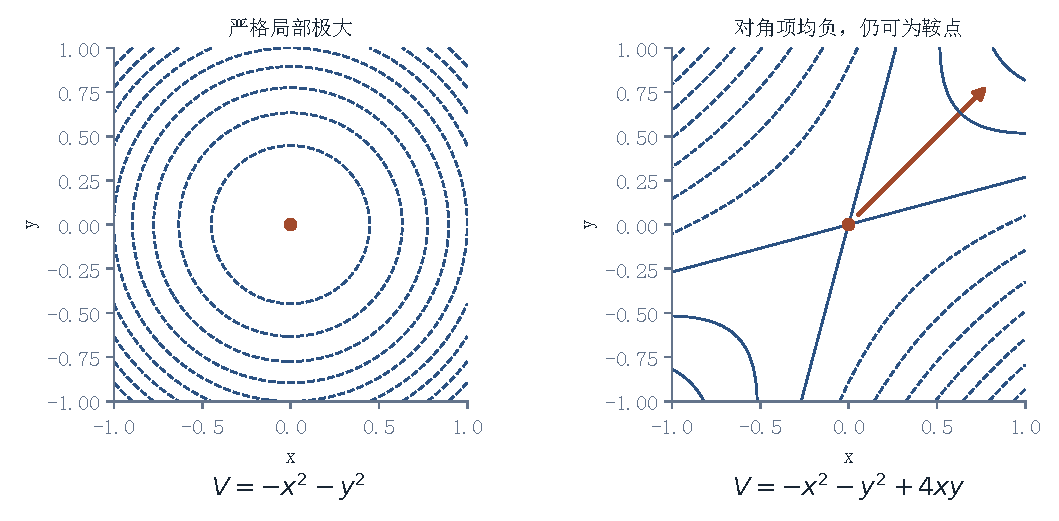
\includegraphics[width=\textwidth]{figures/hessian-directions.pdf}
\caption{两个函数的Hessian对角项均为$-2$。左图为负定，原点是严格局部极大；右图的交叉项使Hessian具有正、负特征值，沿红色方向函数上升，原点成为鞍点。}
\label{fig:mechanism-hessian-directions}
\end{figure}
\subhead{局部最优的三个特征}

停在局部最优上的系统，看上去不像有问题，反而像运行得最好。它可以同时具备三个特征，而这三个特征分别在通常的评价体系里都是正面的。第一是满足度高。系统确实在持续提供用户想要的东西，而且供给效率不断提升。用户的抱怨在减少，因为抱怨的那些点在优化过程中已经被逐条处理掉了。满意度指标好看，留存率好看，增长曲线好看。

第二是稳定。系统不容易被扰动，任何试图改变现状的力量都必须对抗已经形成的整体配置：界面、习惯、商业模式、监管预期、基础设施都已经围绕当前状态调整过，改变一个参数会牵动其他所有参数，成本立刻上升。稳定在这里是一个正面的词，它意味着可预期、可维护、风险低。第三是缺乏生长动力，这一点最难被察觉，因为它不表现为症状。系统没有什么需要解决的问题，也就没有什么需要演化。它的所有改进空间都在当前配置内部：更精细的推荐、更顺滑的交互、更低的延迟。这些改进都在同一条曲线上的平坦区域，边际收益递减，但看起来仍然在进步。

三者叠加的结果是：一个系统可以同时是舒适的、稳定的和停滞的，并且它自己是察觉不到第三项的。这个组合之所以难以纠正，不是因为其中某一项出了问题，而是因为它们互为支撑：正因为满足度高，才没有人有动机去扰动稳定；正因为稳定，才看不到需要解决的问题；正因为看不到问题，改进才会一直沿着平坦区域继续。

\subhead{尼采的末人作为简短对照}

这种处境在思想史上被描述过一次，值得作为对照提出来，但需要把界线划清楚。尼采在《查拉图斯特拉如是说》里写过一个形象，用来描述一种已经放弃了超越的存在：他们不再有渴望，不再有创造，只追求舒适、健康和长寿，并且把这种状态称为幸福。他说这些人“发明了幸福”，然后眨眨眼。\cite{nietzsche1883zarathustra} 这个形象和局部最优的结构有重合，但尼采的批判针对的不是快乐本身，而是当快乐成为唯一目标时，追求更高状态的能力消失了。他的末人不是不幸的，末人恰恰是满足的；问题在于这种满足不再要求任何东西，因此也不产生任何东西。

需要划清的界线在这里。尼采把原因归给价值层面的失败，归给人不再愿意承担更高的目标；局部最优的分析给出的原因更技术化，不是人选择了舒适，而是系统被优化到了舒适的极值点，而在这个点上任何偏离都会立刻降低评价函数的取值。这不是意志问题，是结构问题。人在其中做的每一个决定都可能是理性的，叠加起来却停在一个不再产生新东西的位置上。这个差别的实践含义不小：如果问题是意志，那么解药是呼吁；如果问题是结构，那么解药是改变评价函数本身，而这需要动的是制度、指标和竞争规则，不是个人的决心。

还有一条界线没有划完，而且它比上面那条更要紧。局部最优这个判断本身不含规范内容：系统停在一个极值点上，这件事在结构上是中性的，它是不是失败，取决于评价函数有没有写对。如果评价函数写得正确，那么停在它的最大值上就是成功，不是停滞，而结构分析没有任何工具能把这两种情形分开：它能指出系统不再移动，却指不出这个位置是否值得待。要判定“生长”，必须从结构之外引入一个关于什么算更好的标准，而这个标准不能由同一套优化的语言给出，否则就是循环论证。本章的诊断为停滞准备好了全部机制，没有准备判据；判据是规范问题，不是结构问题，它不能从这里推出来，只能被另外论证。

\subhead{为什么系统不愿离开}

从局部最优离开需要一个特定条件：必须接受一次短期的评价下降，以换取到达另一个更高的局部最优的可能。用形式化的说法，系统需要穿越一段 $V$ 值低于当前水平的地带，这段地带被称为势谷。

\begin{equation}
\Delta V_{\text{escape}} = V(x^*) - \min_{s \in \text{path}} V(s) \ge 0
\label{eq:ch40-escape}
\end{equation}

路径包含起点，因此当前值减去路径最小值非负，表示沿这条路径可能承受的最大暂时评价下降。若要得到到达某个新区域的最小逃逸障碍，还需在允许路径上继续优化。谁承担过渡期的损失、谁获得后续收益，会影响系统是否愿意改变。

个人层面的结构相同，只是承担者换成了自己。一个人要维持某种能力，必须持续使用它，而每一次使用都在当下付出比使用替代方案更高的成本。选择自己写一段文字而不是生成一段，今天的产出更慢、更差；坚持自己去一个地方而不是导航，今天更费时间还可能走错。这些成本是即时的，收益是分散的、延迟的、难以观测的。人的判断系统对即时成本敏感，对延迟收益不敏感，这个偏向在优化充分的低黏滞环境里会被系统性地利用，而且不需要任何人刻意利用它。只要环境提供足够的低摩擦替代品，这个偏向自己就会起作用。

\subhead{停滞不是结局}

把前面的分析收在一起，可以得到一个关于终点的判断。\key{低黏滞陷阱的终点不一定是崩溃，而可能是一个舒适、稳定、缺乏生长动力的局部最优。}系统继续运转，指标继续向好，个体继续得到满足，而整体的可能性空间在收窄。没有人受伤害，没有人抗议，因为确实没有什么可抗议的：系统交付的都是它承诺的东西。收窄发生在另一个维度上，那些需要承受成本才能获得的东西（真实的技能、经过检验的关系、被拒绝过又被坚持下来的判断、一个人自己的边界）不再被生产出来，因为它们的生产过程与当前的评价函数不相容。

这个判断容易被误读成一种文化悲观主义，需要加一句准确的限定。局部最优不是低黏滞环境的必然结果，而是一个需要特定条件才会达到的状态：评价函数必须完全由体验构成，短期反馈必须能够完整地代表长期结果，竞争压力必须有利于最低摩擦方案。当其中某个条件被打破，路径会改变。有大量证据表明现实中的评价函数从来不是完全由体验构成的：身体会出问题，关系会破裂，技能会退化到影响收入，这些长期结果最终会以某种形式回到反馈链上。所以问题不是会不会回来，而是回来的时滞有多长。

时滞决定了代价的分布，也决定了这本书接下来的方向。如果反馈回来的时间很短，个体能在自己的时间尺度上完成校准，代价由自己承担；如果时滞跨越一代人，代价由下一代承担，而承担者没有机会做出不同的选择。这个差别，决定了低黏滞环境是一个可以自我纠正的过程，还是一个只有通过断裂才能纠正的过程。要处理这个问题，需要先看清一件事：人还有哪些能力是系统无法用低成本方式替代的，以及那些能力为什么无法被替代。这个问题在个体身上表现为能力，在群体身上表现为另一种东西：如果大量个体都在同一条路径上适应，那么差异的分布本身也在改变。

\subsection{多样性的丧失与极权心理温床}

前面两节讨论的是个体的边界：拒绝失去对象，系统停在局部最优。这两件事在群体尺度上会合成第三个结果，差异的分布本身发生变化。差异不是抽象的价值，它是边界的原材料。\key{没有差异，就没有可以被拒绝的东西，也没有需要被裁决的冲突。}

\subhead{路径收窄与层流化}

共同的推荐、排序与默认值，可能使许多人暴露于相关的选择路径；用户与网络也可能引入不同方向。群体多样性需要实际测量。流体的层流与湍流不直接给出探索多少、文化好坏或政治倾向的判据，这里的机制应落实到可用替代、共同暴露和纠错能力。

这种收窄的代价已经在别的领域被测量过。金融系统是一个反复出现的例子：同质化程度上升、多样性下降，会让系统更脆弱而不是更鲁棒，当大量机构使用相近的风险模型、持有相近的资产、依赖相近的融资结构时，它们的连接度上升而差异度下降，一个局部冲击因此获得了系统性的放大通道\cite{haldane2011systemic}。农业提供了另一个更早的例子：当一个社会的主粮依赖单一品种时，一次病害就可以穿透整个生产体系，1845 年到 1852 年的爱尔兰马铃薯饥荒属于这一类，单一品种与晚疫病的组合造成约一百万人死亡、约一百万人迁出\cite{ograda1999black}。

这两个例子的共同点不是简化，而是缺少冗余的差异。差异在成本上表现为冗余：多个并行方案、多种做法、看起来多余的选择，都会显得低效。而在扰动到来时，冗余是系统唯一可用的替代路径。低黏滞环境的一个结构性特征，正是它系统性地削掉冗余：既然存在一条最低摩擦的路径，其他路径的使用频率就会下降，最终不再被维护，也不再被练习。

冗余的价值可以用工程上的一个标准来说明。电网运行遵循一条被称为 N-1 的安全准则：系统必须在任何一个元件退出运行之后仍然保持稳定，因此电网必须保有平时看起来多余的容量、备用线路和可调度资源\cite{morison2004power}。这条准则的成本在平时持续发生，收益只在故障时出现，因此它在任何以短期开支为唯一标准的核算里都会被削减。多样性的处境与冗余相同：它表现为成本，兑现为扰动中的存活率，而兑现的时刻在平时看不到。这也是为什么收窄往往不是有人决定收窄，而是没有人有理由为它付账。

这里需要一个重要的边界。把多样性丧失全部归于推荐算法，会错判责任的落点。有研究测量过社交媒体上的跨意识形态接触，结论比流行判断复杂：在 Facebook 的数据中，限制用户接触对立观点的最主要因素是用户自己的朋友构成，算法排序的作用存在，但量级小于前者\cite{bakshy2015exposure}。这个结果的含义不是算法无害，而是收窄有多个来源，把人推向同一路径的力量里，很大一部分来自人自己的选择与网络的同质性。指认正确的机制，是让干预落在有效位置上的前提。

\subhead{秩序的吸引力}

差异被削掉之后，会出现一个看起来无关的心理后果。Arendt的判断在这里可以再往前推一步：她指出极权统治的群众基础是原子化的个体，他们已经失去了阶级、职业共同体和稳定位置的连接；在这样的处境里，孤独比贫困更能解释人们为什么会接受一个把一切事件解释得完全一致的系统\cite{arendt1951origins}。把这个判断与前面两节接起来，可以得到一个更具体的机制：位置消失产生多余感，多余感产生对秩序的需求，而一个持续可用、不犯错、不需要协商的系统，恰好提供了一种廉价的秩序。

这一机制的心理学一侧有可测量的形式。人对自动化系统的信任存在系统性偏差，过度信任与在应当接管时无力接管都会随自动化程度的提高而上升，而这两种失效都不依赖于使用者的知识水平\cite{parasuraman1997humans}。这意味着，交出判断权通常不是一个决定，而是一系列不需要决定的默认：系统给出的答案够用，人工复核显得不必要，几次之后，复核的能力和习惯一起消失。秩序在这里的吸引力不在于它更强，而在于它不需要使用者付出监督成本。

秩序的吸引力还有一层结构原因。一个可解释、可申诉、会出错的秩序，要求使用者承担判断和举证；一个不可解释的秩序把判断收走，同时把责任也收走。对那些已经被判定为多余的个体，交出判断权的收益是双重的：既得到确定性，也免除了为自己判断负责的负担。这也是为什么这种依附很难靠提高警惕来消解，因为它满足的是真实的需求。

依附还有一层更少被提到的收益：它免除了举证的负担。参与一个需要协商的秩序，意味着要说明理由、要面对反驳、要为自己的判断负责；交给一个统一的系统，这些环节全部消失。对那些不确信自己判断能力的人，这种免除是真实的减负，而且它随使用时间增加而加深。这也提示了干预的方向：要维持判断能力，需要的不只是提醒，而是让判断仍然有地方可以提交、有后果可以承担。

把这一步写成必然结局是过度推论。依附的强度取决于替代结构是否存在：如果一个社会仍然保有中间组织，职业共同体、地方关系、长期机构和可以参与的事务，同样的技术压力不会产生同样的依附。技术提供的秩序是可选的，只有当其他秩序来源同时稀薄时，它才成为唯一可得的秩序。分界在这里：不是技术必然导致依附，而是在中间结构被削薄的条件下，依附的成本最低。

三层塌陷到这里合在一处。差异的减少使拒绝失去对象，对象的失去使欲望由外部提供，外部的提供使边界不再由内部维持。这条路径的每一段都在降低下一段的成本，因此它可以被一段接一段地走完，而不需要任何一步是错的。要诊断这条路径，需要的不是道德判断，而是一个能同时容纳三层的结构图。


\begin{figure}[ht]
\centering
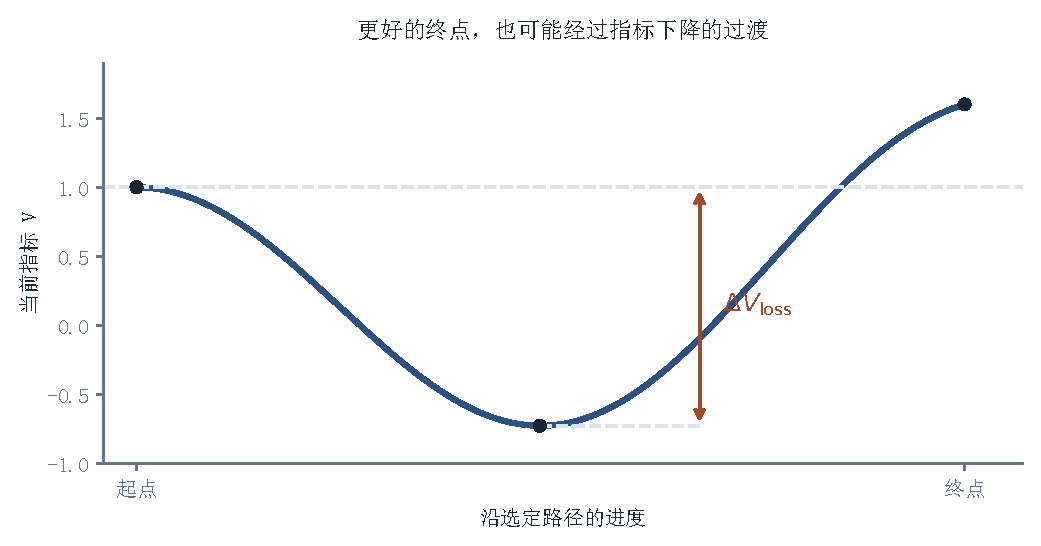
\includegraphics[width=\textwidth]{figures/escape-valley.pdf}
\caption{选定路径上的暂时指标损失。$\Delta V_{\mathrm{loss}}$由起点指标减去该路径上的最小值，因路径包含起点而非负。改变目标、约束或可行路径，会改变这项损失。}
\label{fig:mechanism-escape-valley}
\end{figure}
